\documentclass[12pt, a4paper]{ctexart} % 使用ctexart文档类,支持中文

%%%%%%%%% 页边距设置 %%%%%%%%%
\usepackage{geometry}
\usepackage{graphicx}
\usepackage[english]{babel}
\usepackage{color}
\usepackage{amsmath}
\usepackage{amssymb}
\usepackage{tcolorbox}
\usepackage{listings}
%\usepackage{hyperref}
\input{journal_macros.tex}
\def\tbox#1{\begin{tcolorbox}#1\end{tcolorbox}}
\geometry{a4paper, left=2.5cm, right=2.5cm, top=2.5cm, bottom=2.5cm} % 设置A4纸和页边距

%%%%%%%%% 页眉页脚设置 %%%%%%%%%
\pagestyle{headings}

%%%%%%%%% 超链接设置(使目录可点击) %%%%%%%%%
\usepackage[colorlinks, linkcolor=blue, urlcolor=blue, citecolor=blue]{hyperref}

%%%%%%%%% 文档开始 %%%%%%%%%
\begin{document}
\thispagestyle{empty}
%%%%%%%%% 标题区域 %%%%%%%%%
\title{\Huge \textbf{DroPS}  \\ \huge {\color{blue}D}eriving {\color{blue} $r$} fr{\color{blue}o}m {\color{blue}P}ower {\color{blue}S}pectra}
\author{Zhiqi Huang \\
huangzhq25@mail.sysu.edu.cn}
\date{\today} % 自动显示当前日期,若不需要可改为 \date{}
\maketitle % 生成标题

\thispagestyle{empty} % 标题页不显示页眉页脚
\newpage

%%%%%%%%% 生成目录 %%%%%%%%%
\tableofcontents
\newpage % 目录后换页

%%%%%%%%% 正文内容 %%%%%%%%%
\section{Introduction}


\subsection{Primordial power spectra}
According to the standard cosmological model, the cosmic microwave background (CMB) and the large-scale structure of the universe originated from tiny, nearly Gaussian metric fluctuations in the primordial universe. At linear order, these primordial metric fluctuations can be decomposed into scalar, vector, and tensor modes. Vector perturbations decay rapidly and are therefore generally assumed to be negligible. The primordial scalar and tensor perturbations are respectively parameterized by the dimensionless scalar power spectrum $\mathcal{P}_S(k)$ and tensor power spectrum $\mathcal{P}_T(k)$, where $k$ denotes the comoving wavenumber.

Guided by slow-roll inflation models, the primordial power spectra are commonly parameterized as
\begin{equation}
\mathcal{P}_S(k) = A_s \left(\frac{k}{k{\mathrm{pivot}}}\right)^{n_s - 1},
\end{equation}
and
\begin{equation}
\mathcal{P}_T(k) = r A_s \left(\frac{k}{k{\mathrm{pivot}}}\right)^{n_t}.
\end{equation}
The scalar amplitude $A_s$ and spectral tilt $n_s$ have been tightly constrained by CMB experiments~\cite{Planck18Params}. In most viable inflationary scenarios, the tensor tilt $n_t$ is very small; it is typically either fixed to zero or set to the slow-roll prediction $n_t = -r/8$. The tensor-to-scalar ratio $r$ at the pivot scale, however, remains poorly measured. As of this writing, the best 95\% confidence-level (CL) upper limit is $r < 0.032$~\cite{Tristram22}. Nevertheless, a broad range of inflationary models remains consistent with $0 < r < 0.032$.  

\subsection{CMB B-polarization and $r$}

The search for the signature of primordial gravitational waves in CMB, i.e., measuring $r$ from CMB is one of the most compelling pursuits in modern cosmology. This quest focuses on a unique observable: the B-mode polarization pattern.

The CMB photons became polarized when they scattered off free electrons in the early universe. This process imprinted a directional preference on the light, creating two distinct patterns: E-modes, which have a curl-free pattern like the electric field around charges, and B-modes, which have a curl-like pattern. While density fluctuations (scalar perturbations) in the primordial plasma can generate E-modes and a small amount of B-modes through gravitational lensing (so-called lensing B-modes), they cannot produce the specific, large-scale curl-like pattern of primordial B-modes.

This is where primordial gravitational waves come in. These waves, theorized to be generated during the inflationary epoch, are literally ripples in the fabric of spacetime. As they propagated through the early universe, they periodically stretched and squeezed space, imparting a unique, curl-like distortion to the plasma. This gravitational tugging created a polarization pattern in the CMB that is fundamentally rotational in nature—the primordial B-mode polarization.

Therefore, the B-mode power spectrum at large angular scales acts as a direct tracer for these primordial gravitational waves. A confident detection of this primordial B-mode signal would be tantamount to detecting the gravitational waves themselves. Its amplitude is directly proportional to the energy scale of inflation, with the tensor-to-scalar ratio $r$ quantifying the strength of the signal. Measuring this B-mode power spectrum thus provides a unique window into the physics of the universe's first moments and the grand unification of gravity and quantum mechanics.

\subsection{Ground-based CMB experiments with small-aperture telescopes}

Many ground-based CMB experiments with small-aperture telescopes (SAT), such as BICEP/Keck~\cite{BICEP}, AliCPT~\cite{AliCPT}, and Simons Observatory SAT (SO-SAT)~\cite{SO-SAT} aim to measure the CMB B-mode polarization at degree scales and to constrain the primordial gravitaional waves. These telescopes typically measure the sky emission in the range between $30\mathrm{GHz}$ and $300\mathrm{GHz}$. The raw signals measured by these telescopes are mixture of Galactic foreground, CMB, shot noise, instrumental noise, and contamination from the ground and atmoshpere. Extracting CMB B-mode polarization signal from the mixure of signals is a non-trivial problem and need to be dealt with by specialized softwares. DroPS is one of the software does this job, primarily designed for the ground-based small-aperture telescopes.

\section{Software Documentation}


\subsection{Installing DroPS}

The instruction here has been tested on Ubuntu-24.04.3LTS, and should be easily extendable to other linux platforms. A bit twists may need to be done if you are working with Windows or Mac-OS.

\subsubsection{Installing Tools and Libraries}

Install the following packages and libraries with Synaptic Package Manager (or ``sudo apt install''):

\begin{itemize}
  \item{git}
  \item{gcc}
  \item{gfortran}
  \item{cmake}
  \item{python3-pip}
  \item{python-is-python3}
  \item{python3-venv}
  \item{openmpi-dev}
  \item{libxcb-cursor0}
  \item{libcfitsio-dev}
  \item{libgsl-dev}
  \item{libfftw3-dev}
  \item{libfftw3-mpi-dev}
  \item{libhealpix-dev}
\end{itemize}

\subsubsection{Set up a python virtual environment}

Create a directory for python virtual environment in your work path (hereafter denoted as YourWorkPath)
\tbox{mkdir YourWorkPath/.work}

Create the python virtual environment
\tbox{python  -m  venv YourWorkPath/.work}

Activate the virtual environment
\tbox{source YourWorkPath/.work/bin/activate}
On windows you may need to run
\tbox{YourWorkPath/.work/Scripts/activate.bat}
in cmd.exe or
\tbox{YourWorkPath/.work/Scripts/activate.psl}
in PowerShell.

When you are done with your work, exit the terminal or use
\tbox{deactivate}
to exit the virtual environment.

If you are not working with other python projects. You may want to activate the virtual environment automatically with the terminal 
\tbox{echo ``source YourWorkPath/.work/bin/activate'' \>\> $\sim$/.bashrc}

\subsubsection{Install requirements}


Activate the virtual environment either manually or automatically as described in the previous subsection.

Upgrade pip for the latest information of packages:
\tbox{pip install -\,-upgrade pip}

Now enter your work path where you want to install DroPS
\tbox{cd YourWorkPath}
Get the DroPS repository
\tbox{git clone https://github.com/zqhuang/DroPS}

Now enter the DroPS directory
\tbox{cd DroPS}
Install all dependences
\tbox{pip install -r requirements.txt}

\subsubsection{Hack pysm3}

Hacking a python package is probably against the basic idea of python, but we are doing it anyway to improve the efficiency of CMB simulations. If you only want to analyze maps, however, you can skip this ``unpleasant'' step.

Enter the DroPS directory
\tbox{cd YourWorkPath/DroPS}
Move the cmb.py file in the pysm3 package to somewhere else
\tbox{mv PATH\_TO\_pysm3/models/cmb.py cmb\_backup.py}
and replace it with the cmb.py file that comes with DroPS
\tbox{cp cmb.py PATH\_TO\_pysm3/models/}
Here PATH\_TO\_pysm3 stands for the path where pysm3 was installed. On Ubuntu 24.04.3LTS, you may find PATH\_TO\_pysm3 to be

YourWorkPath/.work/lib/python3.12/site-packages/pysm3

If you are not using Ubuntu24.04.3LTS, the pysm3 path may be slightly different. You can find out the path by doing
\tbox{sudo apt install plocate}
and
\tbox{locate pysm3}


\subsection{Base simulations}

\subsubsection{Generate a TOD filtering model}

A critical step in processing data from ground-based CMB experiments is the removal of contaminating ground and atmospheric signals from the time-ordered data (TOD). To simulate this filtering, one needs specific information about the experiment's site, which is not currently available. Fortunately, the overall effect of the filtering is understood: it suppresses large-scale (low multipole) power in the resulting maps and introduces non-Gaussianity by mixing different Fourier modes.

If you are not keen about simulating precise filtering effect for a specific experiment, you may use the ``mock filtering'' tool that comes with DroPS to generate a filtering matrix:
\tbox{python mock\_filtering.py}

Follow the prompt and enter the healpix resolution (nside, 128 for testing, 256/512 for serious simulations) and the file name for the filtering matrix (e.g. filter\_128.pickle).


\subsubsection{Base simulations}

In this section, we run ``base simulations'' to obtain the statistics of the sky.

To begin with, you can simulate noise/cmb/foreground maps with a 4-channel ground-based experiment
\tbox{python simulate.py Test/test\_sim\_config.txt}
Read the configuration file Test/test\_sim\_config.txt to understand how the experiment is specified.

In this step, you generate a lot of noise and CMB maps based on the noise model and cosmology that are specified in the configuration file.

You also generate a foreground map in this step, based on the model ['d0', 's0'] that is specified in the configuration file. We are not able to generate ``a lot of foreground maps'', as we do not really understand the details of the statistics of the Galactic emission. This ['d0', 's0'] foreground map only captures the gross feature of the Galactic emission. The ``actual foreground'' that we will analyze in the next section can be different from the one in the base simulations.

To understand what ['d0', 's0'] means, follow the pysm3 documentation at \url{https://pysm3.readthedocs.io/}.

\subsection{Analyzing the sky maps}

In the last section, we run ``base simulations'' based on the known noise model, assumed foreground model (['d0', 's0'])  and some assumed $r$ values. In this section, we simulate the ``observed sky'' with the same noise model, optionally a different foreground model, and a $r$ value that has nothing to do with the base simulations. DroPS will reconstruct $r$ by comparing the ``observed sky'' with  the base simulations.

\subsubsection{Analyzing one realization of sky}

Generate the ``observed sky'' with, e.g.,
\tbox{python simulate.py Test/test\_sim\_config.txt maps/test\_  0.01 999}

You can replace maps/test\_ with your preferred prefix for the output maps, 0.01 with your preferred fiducial $r$ value, and 999 with your preferred random seed. To test whether DroPS can deal with a spatial variation of the foreground, you may also replace the ['d0', 's0'] foreground model with ['d1', 's1'] in the configuration file Test/test\_sim\_config.txt.

Now analyze the ``observed sky'' with
\tbox{python mainpipe.py Test/test\_ana\_config.txt maps/test\_}
Read the configuration file Test/test\_ana\_config.txt to understand how to analyze the maps with different settings.

\subsubsection{Analyzing multiple realizations of sky}

In this step we will simulate the sky with may different random seeds, and anlyze all the realizations of sky. The purpose is to test whether the measured $r$ is biased or not.

This time we choose a different foreground model [``d1'', ``s1''] (modify the configuration file Test/test\_sim\_config.txt, if you have not done so). Now run the simulations and analyze them by running the following shell script (test\_bias.sh in the repository)


\begin{lstlisting}[language=bash, caption={Testing $r$ bias}]
#!/bin/bash
for i in `seq 20` 
do 
    python simulate.py Test/test_sim_config.txt maps/test${i}_  0.01 ${i}  d1s1  
    python mainpipe.py Test/test_ana_config.txt maps/test${i}_  Test/r1_logfile_d1s1.txt
done
\end{lstlisting}



Plot the result
\tbox{python utils/plot\_rs.py Test/r1\_logfile\_d1s1.txt 0.01}

Here $0.01$ is the fiducial value of $r$ used in simulations (see the content of test\_bias.sh), used to plot the solid orange line. The mean of reconstructed mean values of $r$ (dotted blue line) is supposed to be close to the fiducial value for an unbiased estimator, as shown in Figure~\ref{fig:r_logs}.

\begin{figure}
  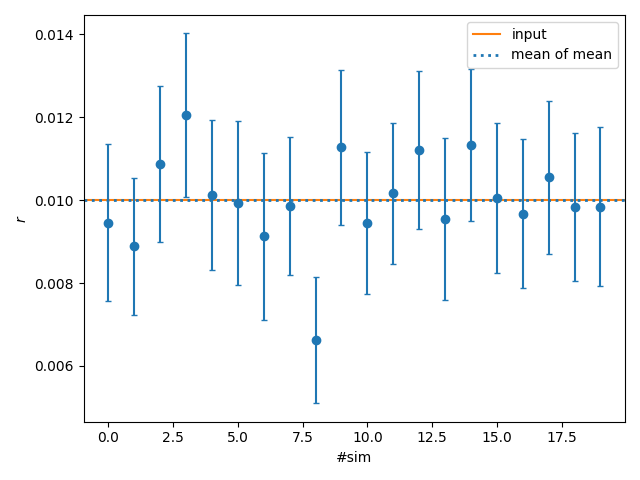
\includegraphics[width=\textwidth]{r_logs.png}
  \caption{Reconstructed $r$ for 20 skys with different random seeds. For each sky, the $r$ value is reconstructed by comparing the sky with 300 simulations. The 20 skys are simulated with foreground model ['d1','s1'] (spatially varying SED of synchrotron and dust emission), while  ['d0', 's0'] (fixed SED) is used in the 300 simulations. \label{fig:r_logs}}
\end{figure}


\subsubsection{How to apply on real data}

A real experiment comes with its own pipeline of noise simulations and TOD filtering, and provides the actually observed sky maps. To analyze the real data, you can simply replace the base simulations with the maps from the simulation pipeline of the experiment, and replace the realization of sky with the actually observed ones.


\subsubsection{Comparing with other pipelines}

DroPS has been applied on AliCPT data challenge (simulated 14\% sky, 95GHz and 150GHz) and achieved consistent results with other methods~\cite{Zhang24}. Here we further compare DroPS with three pipelines that have been applied on simulation data of SO-SAT (Wolz et al. 2024~\cite{SO-SAT}). We adopt the optimistic configuration of SO-SAT. The input fiducial $r$ is zero, and in the analyses unphysical negative $r$ is allowed\footnote{in DroPS this is realized by setting r\_lowerbound negative in the configuration file}.  The results are shown in Figure~\ref{fig:compare_SO}.  From top to bottom, foreground models [``d0'', ``s0''], [``d1'', ``s1''], and [``dm'', ``sm''] are used, respectively. From the left where the reconstructed mean values of $r$ and the bias (mean of the mean values of $r$) are shown, we find DroPS has negligible biases for all cases and more stable than the three pipelines tested in Wolz et al. The right column shows $\sigma_r$, the statistical uncertainties in $r$. We again find good consistency between DroPS and the other pipelines.

\begin{figure}
  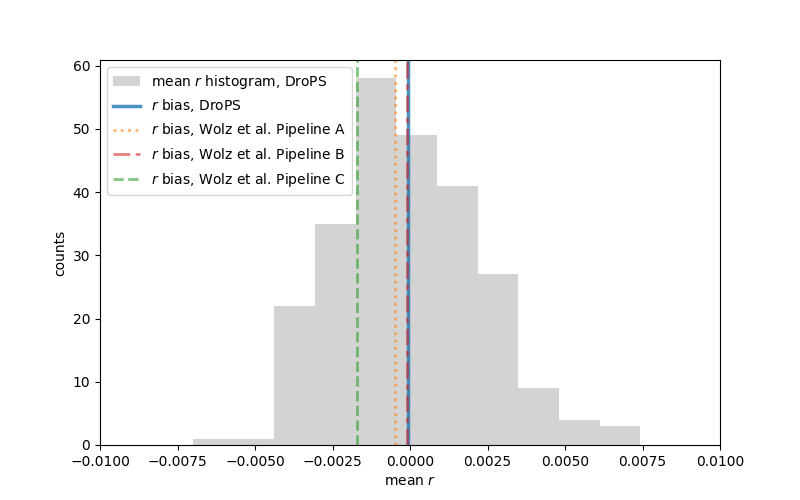
\includegraphics[width=0.5\textwidth]{d0s0_mean.png}%
  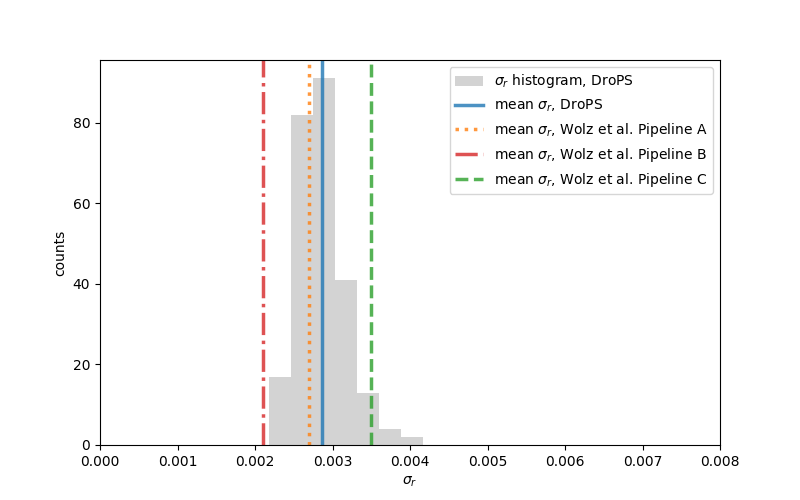
\includegraphics[width=0.5\textwidth]{d0s0_std.png}
  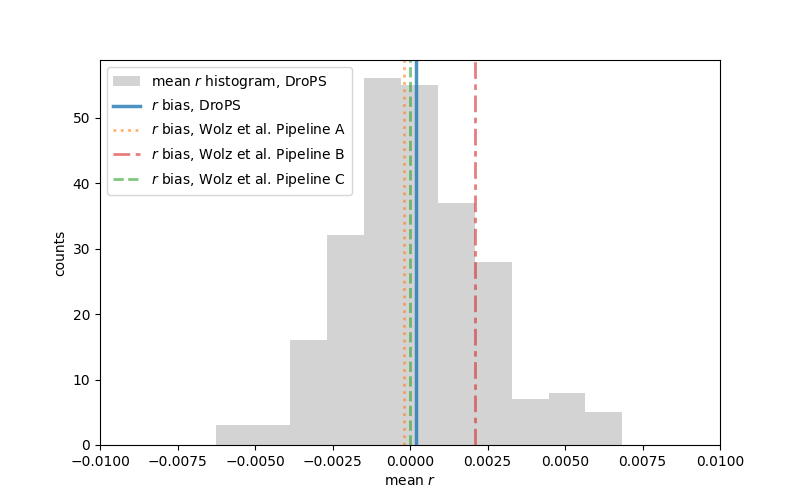
\includegraphics[width=0.5\textwidth]{d1s1_mean.png}%
  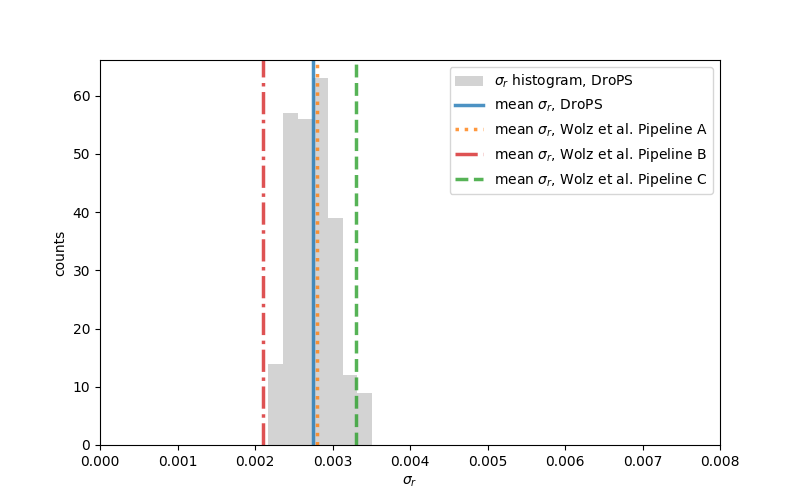
\includegraphics[width=0.5\textwidth]{d1s1_std.png}
  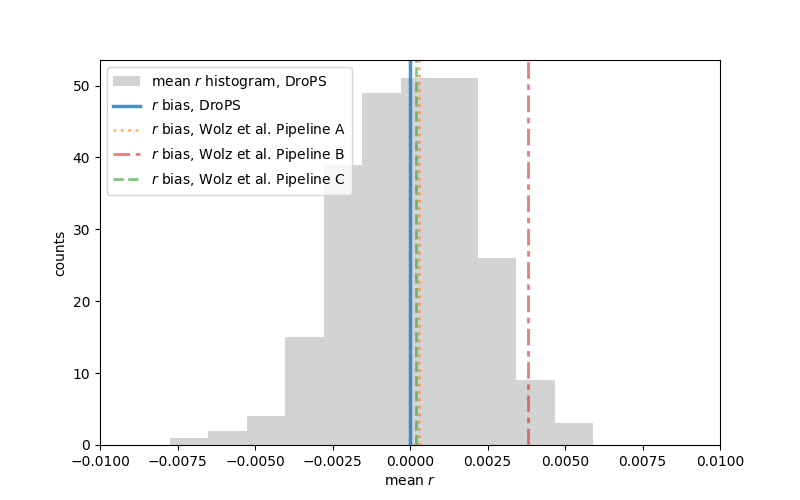
\includegraphics[width=0.5\textwidth]{dmsm_mean.png}%
  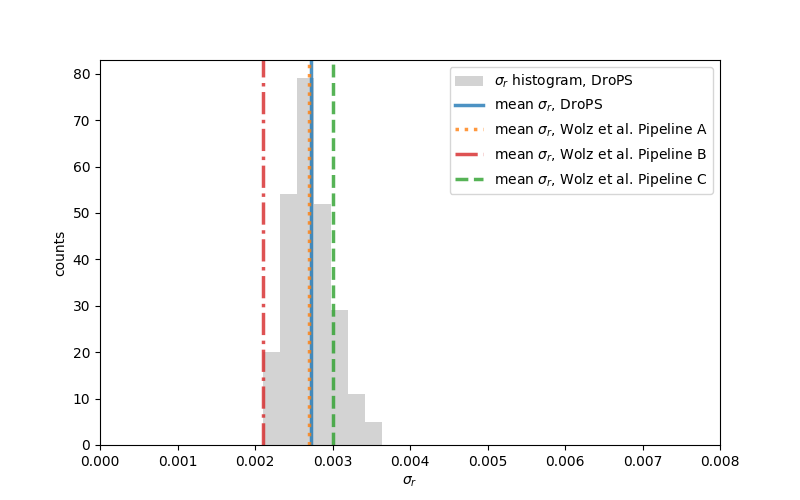
\includegraphics[width=0.5\textwidth]{dmsm_std.png}
  \caption{Comparing DroPS with three pipelines that are described in Wolf et al.~\cite{SO-SAT}. From top to bottom, foreground models ``d0, s0'', ``d1, s1'', and ``dm, sm'' are used, respectively. Left and right columns are the distrubution of reconstructed mean $r$ and $\sigma_r$, respectively.\label{fig:compare_SO}}
\end{figure}

\subsection{Map-level Operations}

\subsubsection{Likelihood-based component separation}

The most well known method of component separation is probably the internal linear combination (ILC) algorithm and its variations. The basic idea is to isolate a signal - whose frequency dependence is known - by taking linear combination of the frequency maps. To do that in pixel space, the frequency maps have to be smoothed to a common resolution. 

For ground-based CMB experiments, however, a key challenge of ILC or ILC-like methods is that TOD filtering and beam convolution are non commutative operations. This prevents the frequency maps from being smoothed to a common resolution. Thus, while ILC remains popular in studies where the complexity of TOD filtering effect is ignored~\cite{SO-SAT}, likelihood-based method - which requires much more computing resources - has been used in real data analyses of BICEP/Keck~\cite{BKmap}.

To demonstrate how the component separation code works, we generate a sky realization from the base simulation \#0:
\tbox{python utils/combine\_sim.py Test/test\_sim\_config.txt maps/r3test0\_  0}
The above script takes the base simulation \#0 and adds the filtered foreground maps, filtered noise maps and filtered cmb maps into sky maps with root name maps/r3test0\_.

Now we do component separation
\tbox{python compsep.py Test/test\_sim\_config.txt maps/r3test0\_}

The code uses Stochastic Gradient Langevin Dynamics (SGLD) method to search the maximum of the likelihood described in Section~\ref{sec:sgld_like}. It typically takes a few days to run compsep.py for the first time, on a personal laptop. When the gradient templates are built, the code runs much faster, typically takes only a few hours on a personal laptop. Typically you need to run it multiple times to obtain a well converged CMB B-mode map. Figure~\ref{fig:compsep} shows the result after four runs of compsep. Due to limited sky coverage and large noise at low-$\ell$, the very low-$\ell$ B-mode does not converge very well. However, the mode at $\ell >50$ are well converged and gives good estimation of the primordial tensor perturbations.

\begin{figure}
  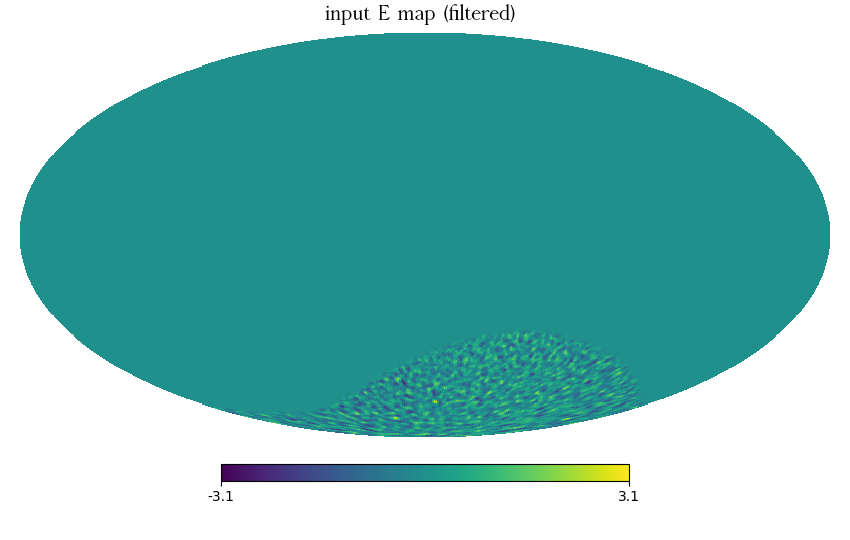
\includegraphics[width=0.5\textwidth]{original_Emap.png}%
  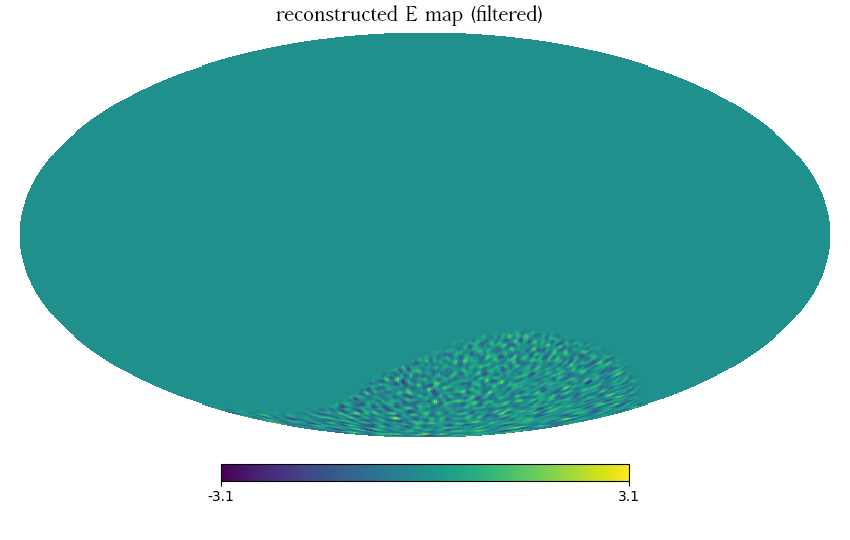
\includegraphics[width=0.5\textwidth]{reconstructed_Emap.png}  
  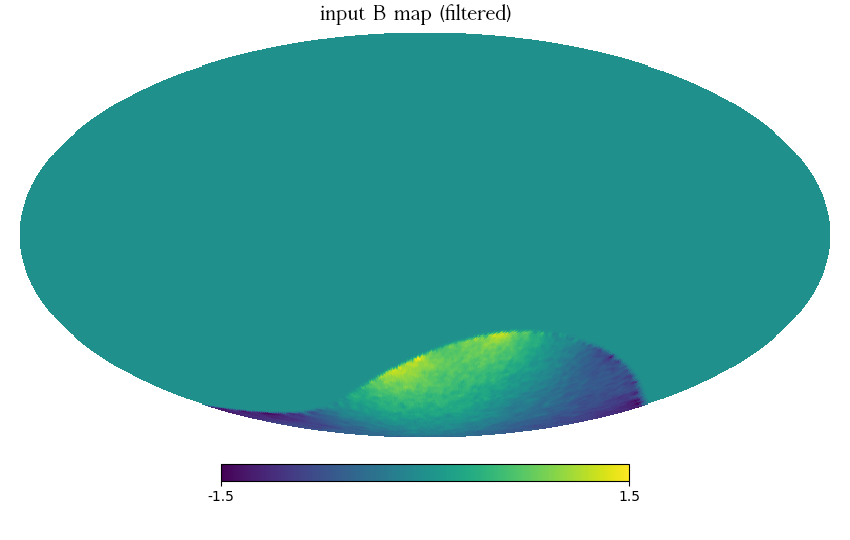
\includegraphics[width=0.5\textwidth]{original_Bmap.png}%
  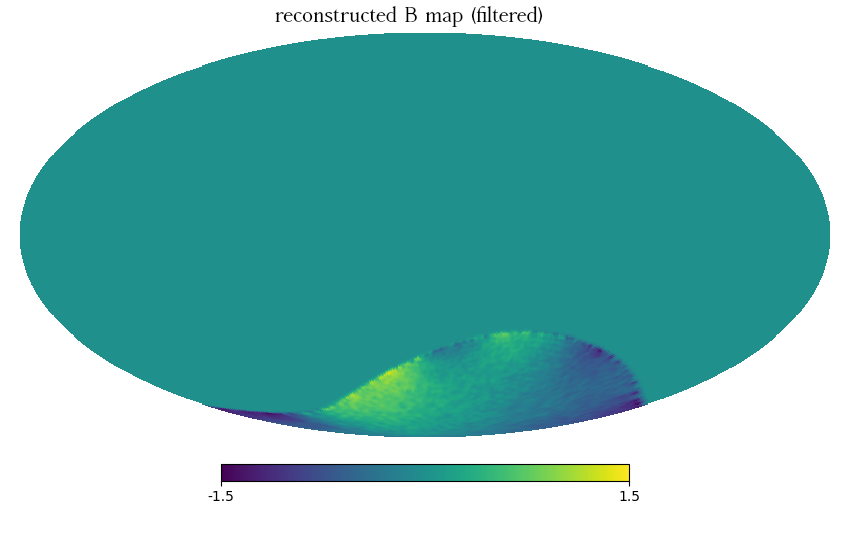
\includegraphics[width=0.5\textwidth]{reconstructed_Bmap.png}  
  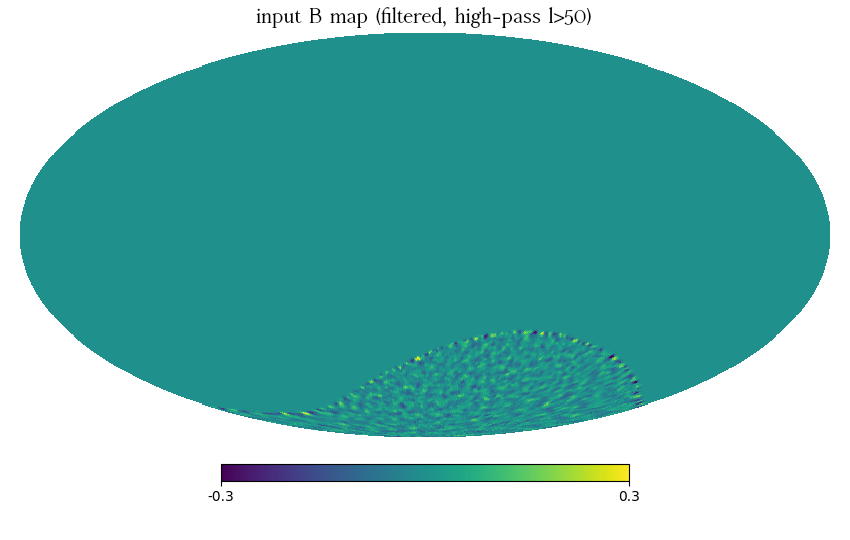
\includegraphics[width=0.5\textwidth]{original_Bmap_l50.png}%
  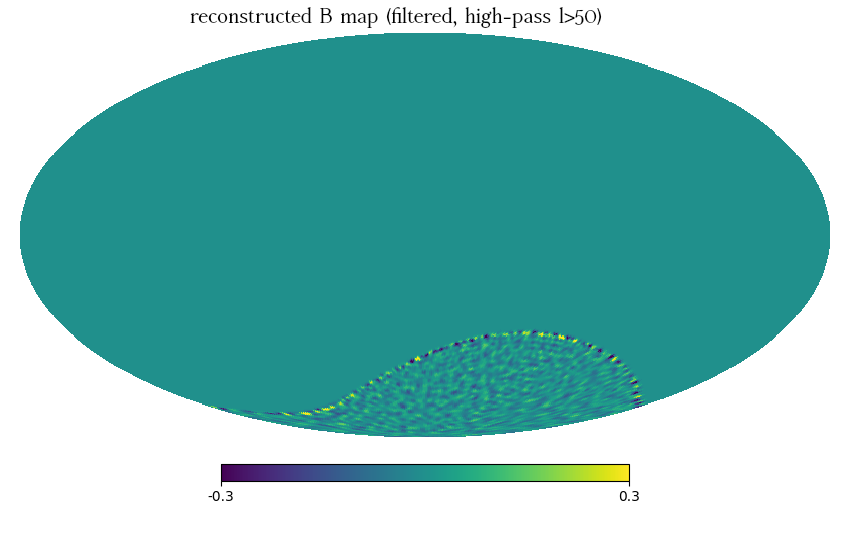
\includegraphics[width=0.5\textwidth]{reconstructed_Bmap_l50.png}
  \caption{Component separation \label{fig:compsep}}
\end{figure}

For real data analyses, the calculation of gradient template involves map making and therefore can take months to built. Fortunately, the gradient template can be built in a parallel way. The template can be built for $\ell \in [\ell_{\min}, \ell_{\max}]$ by running
\tbox{python compsep.py Test/test\_sim\_config.txt maps/r3test0\_ lmin lmax}
Thus, the task can be decomposed into many subtasks with different lmin and lmax. You need $\sim$100GB disk space to store all of these gradient templates.



\subsubsection{Displaying the maps}

DroPS provides a few tools to display the maps: utils/viewfits.py displays the fits map.

\tbox{python utils/viewfits.py NHmask\_G\_128.fits}

If you have a map example\_IQU.fits with I, Q, U components, display the T map with
\tbox{python utils/viewfits.py example\_IQU.fits 0}
and display the Q map with
\tbox{python utils/viewfits.py example\_IQU.fits 1}
display the U map with
\tbox{python utils/viewfits.py example\_IQU.fits 2}


To display maps in npy format, use utils/viewnpy.py.

To display E/B components, use utils/viewEB.py.

\section{Technical Details}

In this section I assume the reader is familiar with Healpix and has the basic knowledge of spherical harmonic analyses.

\subsubsection{TOD filtering}

In ground-based CMB experiments, TOD filtering is a crucial preprocessing step to isolate the faint CMB signal from overwhelming, structured ground-based noise. Since these telescopes observe from the ground, their data streams are heavily contaminated by low-frequency noise, primarily from atmospheric emission and instrumental $1/f$ noise. TOD filtering works in the time domain to identify and subtract these systematic contaminants, which often have characteristic temporal or scan-synchronous patterns distinct from the cosmological CMB fluctuations. By applying high-pass or more sophisticated modal filters, this process effectively suppresses large-scale noise while striving to preserve the intrinsic CMB signal, thereby enabling the recovery of high-fidelity sky maps for cosmological analysis.

Despite being a linear transformation, TOD filtering is typically a dense matrix in both pixel space and harmonic space. DroPS provides an empirical TOD filtering model that captures the following features:
\begin{itemize}
  \item{Significantly suppresses large scale powers.}
  \item{May also slightly suppress small scale powers.}
  \item{Make the map non-Gaussian by mixing different harmonic modes.}      
\end{itemize}
DroPS mimics the TOD filtering effect by joining a few linear processes in both pixel space and in harmonic space. It {\it does not} produce the actual TOD, which would depend on the observational strategy. This allows very quick simulations while keeping the main features of TOD filtering captured.
When
\tbox{python mock\_filtering}
is called. It generates random couping coeffecients between neighboring harmonic modes and save them in a python pickle file that is specified from the command line (e.g., filter\_128.pickle).

When simulating maps, the pickle file is specified in the configuration file (e.g. Test/test\_sim\_config.txt). DroPS loads the pickle file and performs the following linear operations on an input (unfiltered) map.
\begin{itemize}
\item{In pixel space: multiply the input map with a smoothed mask.}
\item{Spherical harmonic transform the map.}  
\item{In harmonic space: mix the harmonic modes with the coupling coefficients loaded from the pickle file.}
\item{Transform back to pixel space.}
\item{Multiply the map with the smoothed mask again.}
\end{itemize}


In the data analyses, DroPS is blind to what has been used in the simulation. It models the filtering effect with a coupling matrix $F_{\ell\ell^\prime}$, whose main diagonal elements describe the suppression effect, sub-diagonal elements describe the coupling between adjacent bins, and all other elements are assumed to be zero. By default, DroPS estimate $F_{\ell\ell'}$ by comparing the band powers of filtered and unfiltered noise maps of the base simulations\footnote{A least square fit is done here.}.

Note that, however, strictly speaking, TOD filtering is a linear operation on the map, but not on the power spectra. The linear modeling may not be very accurate. Consequently, as described in Section~\ref{sec:bandpower_like}, DroPS tends to minimize the usage of the $F_{\ell\ell^\prime}$ matrix.

\subsection{Delensing}


Gravitational lensing by large-scale structure subtly distorts the pristine CMB, smoothing its acoustic peaks and generating a spurious B-mode polarization signal that obscures the far weaker primordial signature. The expectation of CMB lensing B-mode power can be computed from theory and subtracted if the other cosmological parameters are known. However, for actual realization of the universe, the lensing BB power randomly deviate from its expectation value. Such random deviation, often called cosmic variance, which cannot be predicted from the theory may contaminate the measurement of $r$ if we are targeting at $\sigma_r \lesssim 10^{-3}$. Delensing is the process of statistically reconstructing this actual lensing distortion (rather than the theoretical expectation) from high-resolution CMB data itself or from external tracers of the matter distribution, and then removing its effect from the observed CMB map. By cleaning this cosmic foreground, delensing sharpens the CMB's original features and significantly reduces the confounding lensing B-mode power, thereby dramatically improving the sensitivity of experiments to detect the faint imprints of inflation.



\subsection{Likelihood for band powers~\label{sec:bandpower_like}}

DroPS evaluates band powers (average power spectra in $\ell$ bins) of masked maps with NaMaster~\cite{NaMaster}. For measurement of $r$, we typically use a few $\ell$ bins at $20\lesssim \ell \lesssim 200$. Maps with nside = 256 are sufficient for such analyses, and nside = 128 are often good enough for quick estimations. However, if you are changing resolution of maps or rotating them to a different coordinate system, caution should be taken. These operations often leads to extra E-B leakage in low-resolution maps. We recommend nside = 512 for analyses that involve these operations.

The data vector is the band powers of filtered sky maps. The cross correlation between different frequency maps are computed directly, while the auto correlation of a frequency map is computed with pairs of season maps. In all cases, the expectation value of noise band powers are zero. DroPS avoids using auto-correlation of a same map, as the auto correlation of noise can be biased. This is a standard treatment in modern CMB data analyses. 

Suppose the number of $\ell$ bins is $n_{\rm bin}$ and the number of frequency channels is $n_f$. The length of the data vector $D^{XY}_\ell(\nu_1,\nu_2)$ is $N_d=3 n_{\rm bin} n_f(n_f+1)$, if $XY = TT, TE, TB, EE, EB, BB$ band powers are all used. However, since the constraint on $r$ will mostly come from the $BB$ band powers, by default DroPS only uses $BB$ band powers. (This can be changed in the configuration file, e.g., Test/test\_ana\_config.txt.) The default length of data vector is then $N_d = n_{\rm bin}\frac{n_f(n_f+1)}{2}$.  Note that when $\nu_1=\nu_2$,, the band powers are computed by averaging all band powers between season maps,  as we mentioned earlier.

The basic idea is then to compare the data vector $(D_{jk_1k_2})$ with the theory, which include cosmological, foreground, and noise models. The likelihood can be abstractly written as
\begin{equation}
  \mathcal{L} = \frac{1}{(2\pi)^{N_d/2}\sqrt{\det\mathrm{Cov}}} \exp{\left[-\frac{1}{2}(D^{\rm obs} - D^{\rm model})^T\mathrm{Cov}^{-1}(D^{\rm obs} - D^{\rm model})\right]},
\end{equation}
where $D^{\rm obs}$ is the data vector (band powers of observed maps). The model band powers $D^{\rm model}$ can be written as
\begin{equation}
  D^{\rm model} = D^{\rm CMB} + D^{\rm fg},
\end{equation}
where $D^{\rm CMB}$ and $D^{\rm fg}$ are expectation values of band powers of CMB maps and foreground maps, respectively. (The expectation value of noise band powers vanishes as DroPS only takes cross correlations between different frequency bands or between different season maps in a same frequency band.) The covariance $\mathrm{Cov}$ contains the contribution from noise, foreground and CMB. 

\subsubsection{CMB band powers}

The base simulations provide band powers for (filtered and delensed) CMB maps with fiducial $r=0$ and $r=r_1>0$, respectively. The default value of $r_1$ is $0.03$, but you can change it in the configuration file, e.g., Test/test\_sim\_config.txt. Averaging over the base simulations, we obtain the expectation values of CMB band powers $\langle D^{\rm CMB}_\ell(r=0)\rangle $ and $\langle D^{\rm CMB}_\ell(r=r_1)\rangle$.

In the standard cosmological scenario, the band powers has a linear response in $r$ if the other cosmological parameters  (collectively denoted as $\theta$) remain fixed to their fiducial values ($\theta_{\rm fid}$). The CMB band powers are given by
\begin{eqnarray}
  D^{\rm CMB}_\ell &=&  (1-w) \langle D^{\rm CMB}_\ell(r=0)\rangle  + w\langle D^{\rm CMB}_\ell(r=r_1) \rangle \\
  && +\sum_{\ell^\prime} F_{\ell \ell^\prime}\left[D^{\rm CMB}_{\ell^\prime}(r, \theta) - (1-w)D_{\ell^\prime}^{\rm CMB}(r=0, \theta_{\rm fid})- wD_{\ell^\prime }^{\rm CMB}(r=r_1, \theta_{\rm fid})\right],
\end{eqnarray}
where
\begin{equation}
  w \equiv \max\left[\min\left(\frac{r}{r_1}, 1\right), -1\right].
\end{equation}
In other words, DroPS takes the linear interpolation from simulations, which contains all observational effect such as E-to-B leakage, and correct it if $|r|>r_1$ or other cosmological parameters vary. For next generation CMB experiments, the most likely scenario is that $|r|\lesssim r_1$ (as BICEP/Keck data already suggest) and the other cosmological parameters are well constrained. Therefore, the TOD filtering matrix is only applied on a small quantity. This approach minimizes the impact of possibly inaccurate modeling of filtering effect.


\subsubsection{Foreground Model}

The frequency dependence of dust temperature fluctuation is modeled as a modified black-body spectrum, which converted to the CMB $\mu K$ unit is
\begin{equation}
  W_d(\nu) = \left(\frac{\nu}{\nu_{\rm ref}}\right)^{\beta_d-1}e^{\frac{h(\nu_{\rm ref} - \nu)}{k_BT_{\rm CMB}}}\left(\frac{e^{\frac{h\nu}{k_BT_{\rm CMB}}}-1}{e^{\frac{h\nu_{\rm ref}}{k_BT_{\rm CMB}}}-1}\right)^2 \left(\frac{e^{\frac{h\nu_{\rm ref}}{k_BT_{\rm MBB}}}-1}{e^{\frac{h\nu}{k_BT_{\rm MBB}}}-1}\right). \label{eq:dust_w}
\end{equation}
To convert a dust map (in CMB $\mu K$ unit) of frequency $\nu_1$ to dust map at frequency $\nu_2$, a scaling factor $\frac{W_d(\nu_2)}{W_d(\nu_1)}$ is applied.


The frequency dependence of synchrotron temperature fluctuation is modeled as a power-law spectrum, which converted to the CMB $\mu K$ unit is
\begin{equation}
  W_s(\nu) = \left(\frac{\nu}{\nu_{\rm ref}}\right)^{\beta_s-2}e^{\frac{h(\nu_{\rm ref} - \nu)}{k_BT_{\rm CMB}}}\left(\frac{e^{\frac{h\nu}{k_BT_{\rm CMB}}}-1}{e^{\frac{h\nu_{\rm ref}}{k_BT_{\rm CMB}}}-1}\right)^2. \label{eq:sync_w}
\end{equation}
To convert a synchrotron map (in CMB $\mu K$ unit) of frequency $\nu_1$ to dust map at frequency $\nu_2$, a scaling factor $\frac{W_s(\nu_2)}{W_s(\nu_1)}$ is applied.

\subsubsection{Covariance matrix}

\subsection{Likelihood for map-level component separation \label{sec:sgld_like}}

The likelihood $\mathcal{L}\propto e^{-\chi^2/2}$ is based on a Gaussian noise model
\begin{equation}
  \chi^2 = v_{\rm noise}^TN^{-1}v_{\rm noise},
\end{equation}
where $v_{\rm noise}$ is the noise frequency maps inferred from a sky model and the observed frequency maps, and $N$ is the covariance of $v_{\rm noise}$. In pixel space, the size of each vector is $n_{\rm pix} n_f$, i.e., product of the number of pixels and the number of frequency channels. For AliCPT or SO-SAT and maps with degree-scale resolution, we typically have $n_{\rm pixel} n_{\rm frequency} \gtrsim 10^4$. The number of elements in the covariance matrix $N$ is $\gtrsim 10^8$, which is difficult to estimate with simulations and also difficult to invert. The BICEP/Keck analysis~\cite{BKmap} only considers pixel auto-correlation, that is, the diagonal approximation of $N$ in pixel space. A better approximation, which will be used in DroPS, is a diagonal form of $N$ in harmonic space.

We label a pixel with index $j$ ($j=1, 2, \ldots, n_{\rm pix}$), and frequency channels with index $k$ ($k = 1, 2, \ldots, n_f$). The CMB maps are identical in all frequency channels, and are modeled as
\begin{equation}
  (Q\pm \mathrm{i}U)_{\rm CMB, j, k} = -\sum_{\ell = 0}^{\ell_{\max}}\sum_{m=-\ell}^\ell (c_{\ell m}^E\pm \mathrm{i} c_{\ell m}^B)\;_{\pm 2}Y_{\ell m}(\mathbf{n}_j), \label{eq:CMB_comp}
\end{equation}
where $\mathbf{n}_j$ is the directional vector of the $j$-th pixel. Note that here $c_{\ell m}^E$ and $c_{\ell m}^B$ are harmonic coefficients of the full-sky CMB map. Degeneracy between these parameters are expected for partial sky observations. 

Due to limited frequency resolution, BICEP/Keck model $v_{\rm FG}$ as a single component (thermal dust). DroPS takes a more accurate two-component model with emission from Galactic synchrotron and thermal dust. The dust maps are modeled as
\begin{equation}
  (Q\pm \mathrm{i}U)_{\rm dust, j, k} =  -\int W_d(\nu) f_k(\nu) d\nu \,\sum_{\ell = 0}^{\ell_{\max}}\sum_{m=-\ell}^\ell (d_{\ell m}^E\pm \mathrm{i}  d_{\ell m}^B)\;_{\pm 2}Y_{\ell m}(\mathbf{n}_j),  \label{eq:dust_comp}
\end{equation}
where the frequency dependence frunction $W_d$ is defined in Eq.~\eqref{eq:dust_w} and $f_k(\nu)$ is the frequency distribution of the $k$-th frequency channel.
Synchrotron maps are modeled similarly,
\begin{equation}
  (Q\pm \mathrm{i}U)_{\rm sync, j, k} =  -\int W_s(\nu) f_k(\nu) d\nu \,\sum_{\ell = 0}^{\ell_{\max}}\sum_{m=-\ell}^\ell (s_{\ell m}^E\pm \mathrm{i}  s_{\ell m}^B)\;_{\pm 2}Y_{\ell m}(\mathbf{n}_j),  \label{eq:sync_comp}
\end{equation}
where $W_s$ is given in Eq.~\eqref{eq:sync_w}.

The sky model $(Q+iU)_{\rm sky}$ is the sum of Eqs.~(\ref{eq:CMB_comp}, \ref{eq:dust_comp}, \ref{eq:sync_comp}). Passing the sky model through the TOD filtering and map making process, we obtain the filtered sky maps. Substracting the filtered sky maps from the observed (filtered) maps, we obtain filtered noise maps in pixel space. To compute the likelihood, we decompose the noise maps into harmonic space,
\begin{equation}
   M_j(Q\pm \mathrm{i}U)_{\rm noise, filtered, j, k} = -\sum_{\ell = 0}^{\ell_{\max}}\sum_{m=-\ell}^\ell (\tilde{n}_{\ell m}^E\pm \mathrm{i} \tilde{n}_{\ell m}^B)\;_{\pm 2}Y_{\ell m}(\mathbf{n}_j).
\end{equation}
Here $M_j$ is pixel value of a smoothed mask, whose edges are apodized using a C2-type kernel  with an apodization scale of 2 degrees~\cite{Grain09}.  The purpose of introducing such a smoothed mask is to suppress unphysical modes due to sharp-edge and to reduce $E$-to-$B$ leakage.

On the other hand, we can calculate $\tilde{n}_{\ell m}^E$ and $\tilde{n}_{\ell m}^B$ from the filtered noise maps in the base simulations, and compute their diagonal covariance $\tilde{N}^E_{\ell m} \equiv \langle |\tilde{n}_{\ell m}^E|^2\rangle $ and $\tilde{N}^B_{\ell m} \equiv \langle |\tilde{n}_{\ell m}^B|^2\rangle $.

The likelihood $e^{-\chi^2/2}$ is given by
\begin{equation}
  \chi^2 = f_{\rm sky}\sum_{\ell = 0}^{\ell_{\max}} \sum_{m=-\ell}^\ell \frac{|\tilde{n}_{\ell m}|^2}{N_{\ell m}}.
\end{equation}




\bibliographystyle{unsrt}
\bibliography{refs} 

\end{document}
